%%%%%%%%%%%%%%%%%%%%%%%%%%%%%%%%%%%%%%%%%%%%%%
%%%%%%%%%%%%%%%%%%%%%%%%%%%%%%%%%%%%%%%%%%%%%%
%%%%%%%%%%%%%%%%%%%%%%%%%%%%%%%%%%%%%%%%%%%%%%
\chapter{Dark Matter Interaction Rates}
\label{app:interaction_rates}
%%%%%%%%%%%%%%%%%%%%%%%%%%%%%%%%%%%%%%%%%%%%%%
%%%%%%%%%%%%%%%%%%%%%%%%%%%%%%%%%%%%%%%%%%%%%%
%%%%%%%%%%%%%%%%%%%%%%%%%%%%%%%%%%%%%%%%%%%%%%

%%%%%%%%%%%%%%%%%%%%%%%%%%%%%%%%%%%%%%%%%%%%%%
%%%%%%%%%%%%%%%%%%%%%%%%%%%%%%%%%%%%%%%%%%%%%%
\section{General Interaction Rates for Scattering within a Degenerate Media}
\label{app:sec:genral_int_rate}
%%%%%%%%%%%%%%%%%%%%%%%%%%%%%%%%%%%%%%%%%%%%%%
%%%%%%%%%%%%%%%%%%%%%%%%%%%%%%%%%%%%%%%%%%%%%%

The most general form of the interaction rate, following Ref.~\cite{Bertoni:2013bsa_dec_DarkMatterThermalization}, can be written in terms of the spin-averaged squared matrix element, $\Msq$, as
\begin{align}
    \Gamma &= \int\frac{d^3 k'}{(2\pi)^3}\frac{1}{(2E_\chi)(2E_\chi')(2\mi)(2\mi)}\Theta(E_\chi' - \mchi)\Theta(\pm q_0)S(q_0, q),\\
    \begin{split}
        S(q_0, q) & = 2\int\frac{d^3 p}{(2\pi)^3}\int\frac{d^3 p'}{(2\pi)^3}\frac{\mi^2}{\Ei \Ei'}\Msq(2\pi)^4\delta^4\left( k_\mu + p_\mu - k_\mu' - p_\mu'\right)\\
        &\hspace{5em}\times \fFD(\Ei)(1 - \fFD(\Ei'))\Theta(\Ei - \mi)\Theta(\Ei' - \mi),\label{app:eq:full_response_S}
    \end{split}
\end{align}
where $S(q_0, q)$ is the target response function that depends on the energy and momentum transfers, $q_0$ and $q$ respectively.  $E_\chi$ and $\Ei$ are the DM and target initial energies, with $k$ and $p$ their respective momenta. Primed variables represent final state quantities.  

The $\delta$-function can be used to perform the $d^3p'$ integrations, leaving
\begin{equation}
    \begin{split}
        S(q_0, q) = \frac{1}{2\pi^2}\int d^3p \; \frac{\mi^2}{\Ei \Ei'}\Msq &\delta\left( q_0 + \Ei - \Ei'\right) \fFD(\Ei)(1 - \fFD(\Ei'))\\
        &\times\Theta(\Ei- \mi)\Theta(\Ei' - \mi).
    \end{split}
\end{equation}
After this, the final state target energy is fixed to
\begin{align}
    \Ei'(\Ei,q,\theta) &= \sqrt{\mi^2+(\vec{p}+\vec{q})^2}\\
    &= \sqrt{\Ei^2+q^2+2qp\cos\theta} > \mi, \quad\forall p,q,\theta, |\cos\theta|<1,
\end{align}
where $\theta$ is the angle between the target initial momentum and the transferred momentum, $\vec{q}$, that is defined below. To perform the remaining integrals, we write $d^3 p  = p \Ei d\Ei\, d\cos\theta\,d\phi$. The kinematics of this interaction are depicted in Fig.~\ref{app:fig:kin_int_rates}, where the incoming momenta are defined relative to the momentum transfer that is set to lie along the $z$-axis.  In doing so, we must account for the fact that in this frame we cannot assume all three of the vectors are coplanar, and assign the additional azimuthal angle $\phi$ to the target momentum. 

In general, the squared matrix elements we are interested in can be expressed as polynomials in the Mandalstam variables $s$ and $t$, such that
\begin{equation}
    \Msq = \sum_{n,m}\alpha_{n,m} t^n s^m.
\end{equation}
Writing $s = m_\chi^2 + \mi^2 + 2E_\chi \Ei - 2\vec{p}\cdot \vec{k}$, the quantity $\vec{k}\cdot\vec{p}$ is obtained by analysing the kinematics of the interaction. From the diagram in Fig.~\ref{app:fig:kin_int_rates}, we can write the inital momenta as
\begin{align}
    \vec{k} & = (k\sin\theta_\chi, 0, k\cos\theta_\chi),\\
    \vec{p} & = (p\sin\theta \cos\phi, p\sin\theta \sin\phi, p\cos\theta).
\end{align}

\begin{figure}[t!bp]
    \centering
    \begin{tikzpicture}
    \draw[->] (0, -0.5) -- (0, 4) coordinate (s);
    \draw[->] (-4, 0) -- (4, 0) coordinate (x);
    \draw[->] (-4, -1) -- (4,1);
    \draw[dashed, bluemv] (-3,0) -- (-3,2);
    
    \draw[very thick, red, ->] (0,0) coordinate (O) -- (0,3) node [right] {$\vec{q}$};
    \draw[very thick, bluemv, ->] (0,0) -- (-3, 2) coordinate  [label = above:$\vec{k}$] (t);
    \draw[very thick, orangemv, ->] (0,0) -- (2.5, 1.5) coordinate [label = above:$\vec{p}$] (t');
    \draw[dashed, orangemv] (2.5, 1.5) -- (2.5, -1) coordinate (z);
    \draw[dashed, orangemv] (0,0) -- (2.5, -1);
    
    \pic [draw, orangemv,
      angle radius=11mm, angle eccentricity=1.4,
      "$\phi$"] {angle = z--O--x};
      
    \pic [draw, orangemv,
      angle radius=6mm, angle eccentricity=1.4,
      "$\theta$"] {angle = t'--O--s};
      
    \pic [draw, bluemv,
      angle radius=8mm, angle eccentricity=1.4,
      "$\theta_{\chi}$"] {angle = s--O--t};
    \end{tikzpicture}
    \caption{Schematic of kinematics for dark matter interacting with a target in the frame of the star. We set the momentum transfer to lie along the $z$-axis with the initial momenta defined relative to it. }
    \label{app:fig:kin_int_rates}
\end{figure}

The angles can then be expressed in terms of the other kinematic quantities by noting that
\begin{align}
  E'_\chi & = \sqrt{m_\chi^2 + (\vec{k} - \vec{q})},\\
  \implies (E_\chi - q_0)^2  & = m_\chi^2 + (k^2 +q^2 -2 k q \cos\theta_\chi)\\
  \implies \cos\theta_\chi &= \frac{q^2 - q_0^2 +2 E_\chi q_0}{2 q \sqrt{E_\chi^2 - m_\chi^2}},\\
  \Ei' & = \sqrt{\mi^2 + (\vec{p} + \vec{q})},\\
\end{align}
for the dark matter angle, and 
\begin{align}
  \implies (\Ei + q_0)^2  & = \mi^2 + (p^2 +q^2 +2 p q \cos\theta)\\
  \implies \cos\theta &= \frac{q_0^2 - q^2 +2 \Ei q_0}{2 q \sqrt{\Ei^2 - \mi^2}}\label{app:eq:cosn}
\end{align}
for the target angle.
These result in
\begin{align}
    \vec{k}\cdot \vec{p} & = kp\sin\theta_\chi\sin\theta\cos\phi + k p \cos\theta_\chi \cos\theta\\
    \begin{split}
        & = kp\left[ \sqrt{1  - \frac{(q^2 - q_0^2 +2 E_\chi q_0)^2}{4 q^2 (E_\chi^2 - m_\chi^2)}}\sqrt{1 - \frac{(q_0^2 - q^2 +2 \Ei q_0)^2}{4 q^2 (\Ei^2 - \mi^2)}}\cos\phi \right. \\
        &\hspace{6em} \left. + \frac{(q^2 - q_0^2 + 2E_\chi q_0)(q_0^2 - q^2 +2 \Ei q_0)}{4 q^2 \sqrt{E_\chi^2 -m_\chi^2}\sqrt{\Ei^2 -\mi^2}} \right]
    \end{split}\\
    \begin{split}
        & = \frac{(q^2 - q_0^2 + 2E_\chi q_0)(q_0^2 - q^2 +2 \Ei q_0)}{4 q^2}\\ 
        &+ \sqrt{E_\chi^2 - m_\chi^2  - \frac{(q^2 - q_0^2 +2 E_\chi q_0)^2}{4 q^2 }}\sqrt{\Ei^2 - \mi^2 - \frac{(q_0^2 - q^2 +2 \Ei q_0)^2}{4 q^2 }}\cos\phi.
    \end{split}
\end{align}
This makes explicit that $s$ is now a function of the azimuthal angle $\phi$. 

We then use the remaining delta function to integrate over $\theta$, giving rise to a step function $ \Theta(1-\cos^2\theta(q,q_0,\Ei))$, leaving the 
\begin{equation}
S(q_0,q) = \alpha t^n \frac{\mi^2}{2\pi^2 q}\int d\Ei d\phi s^m  \fFD(\Ei)(1-\fFD(\Ei+q_0))\Theta(\Ei)  \Theta(1-\cos^2\theta).
\end{equation}
It will be more convenient to work with the kinetic energies of the targets rather than their total energies, as we are only interested in elastic scattering. From here on out, $\Ei$ will refer to the kinetic energy of the target, i.e. $\Ei\rightarrow \Ei + \mi$. This is compensated by using the Fermi kinetic energy in the FD distributions, $\kinFi = \muFi - \mi$.

The $\phi$ integrals can be easily computed for a given power of $s$, in general resulting in a messy function of the kinematic variables. However, we know that they will always be a polynomial of degree $m$, and so to make this explicit while keeping things as tidy as possible, we define the polynomials $\mathcal{U}_m(q^2, q_0, E_\chi, \Ei)$ as
\begin{equation}
    \mathcal{U}_m = \frac{q^{2m}}{2\pi}\int_0^{2\pi}d\phi\; s^m = \sum_{r}\mathcal{V}_{m,r}\Ei^r
\end{equation}
where the coefficients of the polynomial, $\mathcal{V}_{m,r}$, are functions of $q^2, q_0$, and $E_\chi$.
The response function is then
\begin{equation}
    S(q_0, q) = \alpha t^n \frac{\mi^2}{\pi q}\int d\Ei\; \fFD(\Ei)(1 - \fFD(\Ei +q_0)) \frac{\mathcal{U}_m}{q^{2m}}\Theta(\Ei)\Theta(1 - \cos^2\theta).
\end{equation}

Therefore, the integrals we are interested in computing are over the FD distributions, which we call
\begin{equation}
    \mathcal{F}_r(\Ei, q_0) = \int d\Ei \Ei^r \fFD(\Ei)(1 - \fFD(\Ei + q_0)).
\end{equation}
To proceed, make the change to the dimensionless variables
\begin{equation}
    x = \frac{\Ei - \kinFi}{\Tstar}, \; z = \frac{q_0}{\Tstar},
\end{equation}
which we can use to write
\begin{align}
       \mathcal{F}_r(E_i, q_0) & = \Tstar\int dx \left( \kinFi + \Tstar x\right)^r \fFD(x)\fFD(-x-z)\\
       & = \Tstar\int dx \sum_{j = 0}^r \binom{r}{j} \Tstar^j x^j \kinFi^{r-j}\fFD(x)\fFD(-x-z)\\
       & = \sum_{j = 0}^r \Tstar^{j+1} \binom{r}{j}\kinFi^{r-j}\int dx x^j\fFD(x)\fFD(-x-z)\\
       & =  \sum_{j = 0}^r \binom{r}{j} \kinFi^{r-j} \int d\Ei (\Ei - \kinFi)^j \fFD(\Ei)\fFD(-\Ei - q_0)\\ 
    %   & = \sum_{j = 0}^r \binom{r}{j} \kinFi^{r-j} F_j(\Ei -\kinFi, q_0)\\
       & = \sum_{j = 0}^r \binom{r}{j} \kinFi^{r-j} (-1)^{j} \frac{q_0^{j+1}}{j+1}g_j\left( \frac{\Ei - \kinFi}{q_0} \right),\quad\mathrm{for}\; \Tstar\rightarrow 0,
\end{align}
where the final line holds in the zero-temperature approximation in which the FD distributions become $\Theta$-functions, allowing the integrals to be expressed in terms of the function 
\begin{equation}
    g_j(x) = \begin{cases}
        & 1, \quad x >0\\
        & 1-(-x)^{j+1},\quad -1<x <0\\
        & 0,\quad x<-1
    \end{cases}.
\end{equation}
% For $i = 1, 2$ we have
% \begin{align}
%     \int d\Ei \Ei \fFD(\Ei)(1 - \fFD(\Ei + q_0)) & =F_1(\Ei -\kinFi, q_0) + \kinFi F_0(\Ei -\kinFi, q_0)\\
%     \int d\Ei \Ei^2 \fFD(\Ei)(1 - \fFD(\Ei + q_0)) & = F_2(\Ei -\kinFi, q_0) + 2\kinFi F_1(\Ei -\kinFi, q_0) + \kinFi^2 F_0(\Ei -\kinFi, q_0)
% \end{align}

The integration range for $\Ei$ is obtained from the two $\Theta$-functions. There are two cases to be considered, $t<0$ and $t>0$. In the former case, the range become $\Ei^{t^-}<\Ei<\infty$ and for the latter $0<\Ei<\Ei^{t^+}$. These integration bounds are obtained from Eq.~\ref{app:eq:cosn}, by settting $\cos\theta = 1$, and are given by
\begin{align}
    \Ei^{t^-} & = -\left( \mi+\frac{q_0}{2}\right) + \sqrt{\left( \mi+\frac{q_0}{2}\right)^2 + \left( \frac{\sqrt{q^2 - q_0^2}}{2} - \frac{\mi q_0}{\sqrt{q^2 - q_0^2}}\right)^2}\\
    \Ei^{t^+} & = -\left( \mi+\frac{q_0}{2}\right) + \sqrt{\left( \mi+\frac{q_0}{2}\right)^2 - \left( \frac{\sqrt{q_0^2 - q^2}}{2} + \frac{\mi q_0}{\sqrt{q_0^2 - q^2}}\right)^2}.
\end{align}
These are both the same root of Eq.~\ref{app:eq:cosn}, but with an interchange of $t\leftrightarrow -t$. We denote the response function for $t<0$ as $S^-$ and for $t>0$ as $S^+$. For $S^-$ we have
\begin{align}
    S^-_m & = \alpha t^n \frac{\mi^2}{\pi q^{2m + 1}}\sum_{r=0}^m \mathcal{V}_{m,r}\int_{\Ei^{t^-}}^\infty d\Ei \Ei^r \fFD(\Ei)(1 - \fFD(\Ei +q_0))\\
    & = \alpha t^n \frac{\mi^2}{\pi q^{2m + 1}}\sum_{r=0}^m \mathcal{V}_{m,r} \sum_{j = 0}^r \binom{r}{j} \kinFi^{r-j}\int_{\Ei^{t^-}}^\infty d\Ei (\Ei - \kinFi)^j \fFD(\Ei)\fFD(-\Ei - q_0)\\
    & =  \alpha t^n \frac{\mi^2}{\pi q^{2m + 1}}\sum_{r=0}^m \mathcal{V}_{m,r} \sum_{j = 0}^r \binom{r}{j} \kinFi^{r-j}  \frac{(-1)^{j} q_0^{j+1}}{j+1}\left[ 1 - g_j\left( \frac{\Ei^{t^-} - \kinFi}{q_0}\right) \right]\\
    & =  \alpha t^n \frac{\mi^2}{\pi q^{2m + 1}}\sum_{r=0}^m \mathcal{V}_{m,r} \sum_{j = 0}^r \binom{r}{j} \kinFi^{r-j}  \frac{(-1)^{j} q_0^{j+1}}{j+1} h_j\left( \frac{\Ei^{t^-} - \kinFi}{q_0}\right),
\end{align}
while for $S^+$ the logic is
\begin{align}
    S^+_m & = \alpha t^n \frac{\mi^2}{\pi q^{2m + 1}}\sum_{r=0}^m \mathcal{V}_{m,r}\int_{0}^{\Ei^{t^+}} d\Ei \Ei^r \fFD(\Ei)(1 - \fFD(\Ei +q_0))\\
    & = \alpha t^n \frac{\mi^2}{\pi q^{2m + 1}}\sum_{r=0}^m \mathcal{V}_{m,r} \sum_{j = 0}^r \binom{r}{j} \kinFi^{r-j}\int_{0}^{\Ei^{t^+}} d\Ei (\Ei - \kinFi)^j \fFD(\Ei)\fFD(-\Ei - q_0)\\
    & =  \alpha t^n \frac{\mi^2}{\pi q^{2m + 1}}\sum_{r=0}^m \mathcal{V}_{m,r} \sum_{j = 0}^r \binom{r}{j} \kinFi^{r-j}  \frac{(-1)^{j} q_0^{j+1}}{j+1}\left[ g_j\left( \frac{\Ei^{t^+} - \kinFi}{q_0}\right) -  g_j\left( \frac{ - \kinFi}{q_0}\right) \right]\\
    & =  -\alpha t^n \frac{\mi^2}{\pi q^{2m + 1}}\sum_{r=0}^m \mathcal{V}_{m,r} \sum_{j = 0}^r \binom{r}{j} \kinFi^{r-j}  \frac{(-1)^{j} q_0^{j+1}}{j+1} h_j\left( \frac{\Ei^{t^+} - \kinFi}{q_0}\right)\quad \textrm{for}\; q_0<0,
\end{align}
with 
\begin{equation}
    h_j(x) = \begin{cases}
        & 0, \quad x >0\\
        & (-x)^{j+1},\quad -1<x <0\\
        & 1,\quad x<-1
    \end{cases}.
\end{equation}

The final step of the $S^+$ calculation holds only for up-scattering of the DM, i.e. $q_0<0$.
% Some results
% \begin{align}
%      S_0 &= \alpha t^n \frac{\mi^2 q_0}{\pi q}h_0\left( \frac{\Ei^{t^-} - \kinFi}{q_0}\right)\\
%      S_1 &= \alpha t^n \frac{\mi^2}{\pi q^3}\left[ \mathcal{V}_{1,0} \left( q_0 h_0\left( \frac{\Ei^{t^-} - \kinFi}{q_0}\right) \right) + \mathcal{V}_{1,1} \left( \kinFi q_0 h_0\left( \frac{\Ei^{t^-} - \kinFi}{q_0}\right) -\frac{q_0^2}{2}h_1\left( \frac{\Ei^{t^-} - \kinFi}{q_0}\right)  \right)\right]
% \end{align}

For matrix elements that are polynomials in $s$ and $t$, the full response function is simply the sum of the $n$ and $m$, giving
\begin{align}
    S^- & = \sum_{n,m}\alpha_{n,m} t^n \frac{\mi^2}{\pi q^{2m + 1}}\sum_{r=0}^m \mathcal{V}_{m,r} \sum_{j = 0}^r \binom{r}{j} \kinFi^{r-j}  \frac{(-1)^{j} q_0^{j+1}}{j+1} h_j\left( \frac{\Ei^{t^-} - \kinFi}{q_0}\right)\\
    S^+ & = -\sum_{n,m}\alpha_{n,m} t^n \frac{\mi^2}{\pi q^{2m + 1}}\sum_{r=0}^m \mathcal{V}_{m,r} \sum_{j = 0}^r \binom{r}{j} \kinFi^{r-j}  \frac{(-1)^{j} q_0^{j+1}}{j+1} h_j\left( \frac{\Ei^{t^+} - \kinFi}{q_0}\right)
\end{align}

%%%%%%%%%%%%%%%%%%%%%%%%%%%%%%%%%%%%%%%%%%%
%%%%%%%%%%%%%%%%%%%%%%%%%%%%%%%%%%%%%%%%%%%
\section{Elsatic Scattering}
\label{app:sec:elastic_scatter_full}
%%%%%%%%%%%%%%%%%%%%%%%%%%%%%%%%%%%%%%%%%%%
%%%%%%%%%%%%%%%%%%%%%%%%%%%%%%%%%%%%%%%%%%%

%%%%%%%%%%%%%%%%%%%%%%%%%%%%%%%%%%%%%%%%%%%
\subsection{Down-scattering Rate}
\label{app:subsec:down_scatter_derivation}
%%%%%%%%%%%%%%%%%%%%%%%%%%%%%%%%%%%%%%%%%%%

Returning to the scattering rate, we first look at the case of down-scattering, where the DM loses energy, $q_0 > 0$. In this case, the interaction rate is given by
\begin{equation}
    \begin{split}
        \Gamma^{-}(E_\chi) = \int \frac{d\cos\theta_\chi k^{'2}dk'}{64\pi^3 E_\chi E'_\chi } & \Theta(E_\chi-q_0-m_\chi)\Theta(q_0)\sum_{n,m} \frac{\alpha_{n,m} t^n}{ q^{2m + 1}}\\
        &\times \sum_{r=0}^m \mathcal{V}_{m,r} \sum_{j = 0}^r \binom{r}{j} \kinFi^{r-j}  \frac{(-1)^{j} q_0^{j+1}}{j+1} h_j\left( \frac{\Ei^{t^-} - \kinFi}{q_0}\right)
    \end{split}
\end{equation}
Change variables to $q_0$ and $q$ through
\begin{align}
    q_0 &= E_\chi - \sqrt{k'^2 +m_\chi^2},\\
    q^2 &= k^2 + k'^2 -2kk'\cos\theta_\chi,\\
    \implies dk' d\cos\theta_\chi  & = \frac{E_\chi' q}{kk'^2} dq_0 dq
\end{align}
To further simplify the notation we introduce $t_E = -t = q^2 - q_0^2$, $dq = dt_E/(2q)$, and exchange the $q$-integral for
\begin{equation}
    \implies dk' d\cos\theta_\chi = \frac{E_\chi' }{2kk'^2} dq_0 dt_E,
\end{equation}
giving the interaction rate as
\begin{align}
    \begin{split}
        \Gamma^{-}(E_\chi)- & = \frac{1}{128\pi^3 E_\chi k }\int_0^{E_\chi -m_\chi} dq_0 \int dt_E\sum_{n,m} \frac{\alpha_{n,m} (-1)^n t_E^n}{ (t_E+q_0^2)^{m + \frac{1}{2}}}\\
        &\hspace{4em}\times\sum_{r=0}^m \mathcal{V}_{m,r} \sum_{j = 0}^r \binom{r}{j} \kinFi^{r-j}  \frac{(-1)^{j} q_0^{j+1}}{j+1} h_j\left( \frac{\Ei^{t^-} - \kinFi}{q_0}\right)
    \end{split}\\
    \begin{split}
        & = \sum_{n,m}  \frac{(-1)^n \alpha_{n,m}}{128\pi^3 E_\chi k }\int_0^{E_\chi -m_\chi} dq_0\int \frac{dt_E t_E^n}{(t_E + q_0^2)^{m+\frac{1}{2}}}\\
        &\hspace{4em}\times\sum_{r=0}^m \mathcal{V}_{m,r}\sum_{j = 0}^r\binom{r}{j} \kinFi^{r-j}  \frac{(-1)^{j} q_0^{j+1}}{j+1} h_j\left( \frac{\Ei^{t^-} - \kinFi}{q_0}\right)
    \end{split}.
    % \\
    % \Gamma^+ & = \sum_{n,m}  \frac{ \alpha_{n,m}}{128\pi^3 E_\chi k }\int_{-\infty}^0 dq_0 \int \frac{dt\; t^n}{(q_0^2 - t)^{m+\frac{1}{2}}}\sum_{r=0}^m \mathcal{V}_{m,r}\sum_{j = 0}^r\binom{r}{j} \kinFi^{r-j}  \frac{(-1)^{j} q_0^{j+1}}{j+1} h_j\left( \frac{\Ei^{t^+} - \kinFi}{q_0}\right)
\end{align}

There are then two main cases to consider; when $h_j(x)$ is unity or when it is not. We denote the $t_E$ integrand in the former case as $f_1$ and $f_2$ for the latter, given explicitly as
\begin{align}
    f_1^{(m,n)}(t_E) & =  \frac{t_E^n}{(t_E + q_0^2)^{m+\frac{1}{2}}}\sum_{r=0}^m \mathcal{V}_{m,r}\sum_{j = 0}^r\binom{r}{j} \kinFi^{r-j}  \frac{(-1)^{j} q_0^{j+1}}{j+1},\\
    f_2^{(m,n)}(t_E) & = \frac{-t_E^n}{(t_E + q_0^2)^{m+\frac{1}{2}}}\sum_{r=0}^m \mathcal{V}_{m,r}\sum_{j = 0}^r\binom{r}{j} \kinFi^{r-j}  \frac{1}{j+1} \left( \Ei^{t^-} - \kinFi\right)^{j+1},
\end{align}
where we suppress the explicit dependence on the other variables for brevity. We encode the integrals over $t_E$ within an operator 
\begin{align}
    \begin{split}
        \mathcal{I}_{n,m}(f^{(m,n)}(t),t_1^+,t_2^+,t_1^-,t_2^-) &= \sum_{i=1,2}\sum_{j=1,2} \left(F^{(m,n)}(t_i^+)-F^{(m,n)}(t_j^-)\right)\\
        &\hspace{2em}\times \Theta\left(t_{3-i}^+-t_i^+\right)\Theta\left(t_i^+-t_j^-\right)\Theta\left(t_j^--t_{3-j}^-\right),
    \end{split}\\
    F^{(m,n)}(t) &= \int dt \, f^{(m,n)}(t).
\end{align}

The full interaction rate is then written as
\begin{align}
    \begin{split}
        \Gamma^{-}(E_\chi)  =& \sum_{n,m}  \frac{(-1)^n \alpha_{n,m}}{128\pi^3 E_\chi k }\int_0^{E_\chi -m_\chi} dq_0  \\
         \times & \left[ \mathcal{I}_{n,m}\left(f_1^{(m,n)}(t),t_E^+,t_{\mu^-}^+,t_E^-,t_{\mu^-}^-\right)\Theta(\kinFi-q_0)\right.\\
        + & \mathcal{I}_{n,m}\left(f_2^{(m,n)}(t),t_E^+,t_{\mu^+}^+,t_E^-,t_{\mu^-}^+\right)\Theta(\kinFi-q_0) \\
        + & \mathcal{I}_{n,m}\left(f_2^{(m,n)}(t),t_E^+,t_{\mu^-}^-,t_E^-,t_{\mu^+}^-\right)\Theta(\kinFi-q_0) \\
        + & \left. \mathcal{I}_{n,m}\left(f_2^{(m,n)}(t),t_E^+,t_{\mu^+}^+,t_E^-,t_{\mu^+}^-\right)\Theta(q_0-\kinFi) \right], \label{app:eq:gammafull_app}
    \end{split}
\end{align}
where the $t_E$ integration limits are
\begin{align}
 t_E^\pm &= 2\left[E_\chi(E_\chi-q_0)-m_\chi^2\pm k\sqrt{(E_\chi-q_0)^2-m_\chi^2}\right],\\
 \begin{split}
    t_{\mu^{+}}^\pm &= 2\left[\kinFi(\kinFi+q_0)+\mi(2\kinFi+q_0) \right. \\
    &\hspace{4em}\left.\pm \sqrt{\left(\kinFi(\kinFi+q_0)+\mi(2\kinFi+q_0)\right)^2-\mi^2q_0^2}\right],
 \end{split}\\
 \begin{split}
    t_{\mu^{-}}^\pm &=  2\left[\kinFi(\kinFi-q_0)+\mi(2\kinFi-q_0)\right.\\
    &\hspace{4em}\left.\pm\sqrt{\left(\kinFi(\kinFi-q_0)+\mi(2\kinFi-q_0)\right)^2-\mi^2q_0^2}\right], 
 \end{split}
\end{align}

All interaction rate spectra will have an endpoint at $q_0 = \qomax$, the maximum amount of energy that can be lost in a single interaction.
The value of $\qomax$ is shown in the left panel of Fig.~\ref{ch3:fig:q0max} as a function of $B$ in the case of large DM mass ($m_\chi = 1\TeV$), for several values of $\kinFn$. The endpoint can be found as the minimum between the DM kinetic energy and the root of one of the following two equations 
\begin{align}
    t_E^- &= t_{\mu^+}^+,\\
    t_E^+ &= t_{\mu^+}^-.
\end{align}
Only one of these equations will have a positive root for a given choice of $m_\chi$, $\kinFn$ and $E_\chi$.
For $m_\chi\gg \mi$, the second equation never has a solution, and the solution of the first equation is always much lower than the kinetic energy. This results in the value of $\qomax$ becoming independent of $m_\chi$ in this mass range.


The shape of the differential interaction rate depends very weakly on $m_\chi$ and $B$ for $m_\chi\gg \mi$ and $m_\chi \ll \mi$, as seen by plotting it as a function of $\qonorm=q_0/\qomax$. Therefore, we use as a reference $m_\chi=1\TeV$ (left) and $m_\chi=10\MeV$ (right),  $B=0.5$, and show the normalised differential interaction rates in Fig.~\ref{app:fig:diffgamma} for $n=0,1,2$, and neutron targets.
We observe in the left panels that for $n=0$ interaction rates are flat (or peaked, depending on $\kinFn$) at low energy and suppressed at high energies, while for $n=1,2$ the profiles become peaked at higher and higher energies. Conversely, for $m_\chi=10\MeV$ the peak of the spectrum is shifted to lower energies with increasing power of $t$ ($d\sigma\propto t^n$).

\begin{figure}
    \centering
    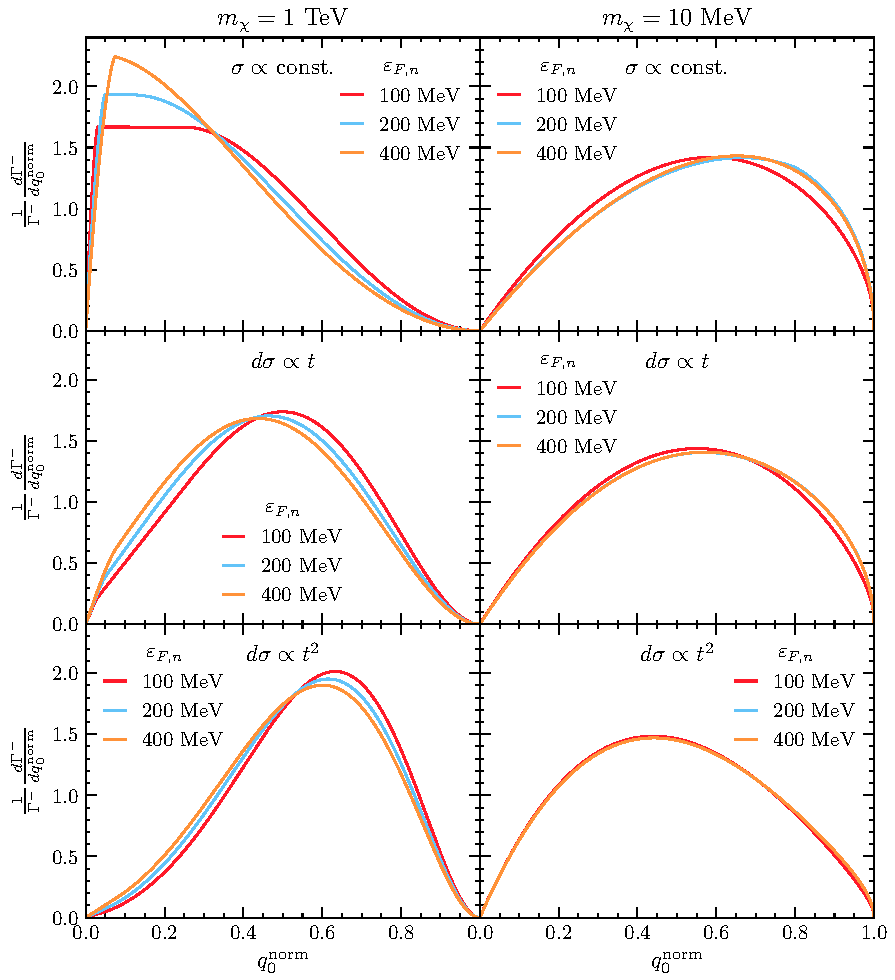
\includegraphics[width = 0.85\textwidth]{img/capture_intro/capture_1/norm_diff_intrate_n.pdf}
    \caption{Normalised differential interaction rates, $\frac{1}{\Gamma}\frac{d\Gamma^-}{d\qonorm}$, as a function of $\qonorm$ for different values of $\kinFn$, with $m_\chi=1\TeV$ (left panels) $m_\chi=10\MeV$ (right panels) and $B=0.5$. Top row: $n=0$, middle row: $n=1$, bottom row: $n=2$.}
    \label{app:fig:diffgamma}
\end{figure}

%%%%%%%%%%%%%%%%%%%%%%%%%%%%%%%%%%%%%%%%%%%
\subsection{Up-scattering Rate}
\label{app:subsec:up_scatter_derivation}
%%%%%%%%%%%%%%%%%%%%%%%%%%%%%%%%%%%%%%%%%%%

We now treat the case of $q_0<0$, applicable to up scattering and evaporation. Focusing on $s$-independent matrix elements for the moment, the response function is
\begin{equation}
    S^{-}_\mathrm{up}(q_0, q) = \frac{\mi^2}{\pi q}\int_{\Ei^{t^-}}^\infty\fFD(\Ei)(1 - \fFD(\Ei -|q_0|))
\end{equation}
and evaluate the integral, now with $q_0 <0$. If we attempt to take the $\Tstar\rightarrow 0$ limit as before, we find that there is no overlap of the FD distributions and the result vanishes. Instead, we keep the leading order thermal corrections, i.e. terms of order $e^{-|q_0|/\Tstar}$. The result is 
\begin{equation}
        \mathcal{F}_0(\Ei, -|q_0|) = \frac{\Tstar e^{-|q_0|/\Tstar}}{1 - e^{-|q_0|/\Tstar}} \left[ \log\left( 1 + e^{(\Ei-\kinFi)/\Tstar}\right) - \log\left( 1 + e^{(\Ei-|q_0|-\kinFi)/\Tstar}\right)\right],
\end{equation}
where after taking $\Tstar \rightarrow 0$ we recognise three regions of interest
\begin{equation}
    \lim_{\Tstar \rightarrow 0}\Tstar \mathcal{F}_0(\Ei, -|q_0|) = 
    \begin{dcases}
        \frac{|q_0| e^{-|q_0|/\Tstar}}{1 - e^{-|q_0|/\Tstar}},&\quad \Ei>\kinFi +|q_0|\\  
        \frac{(\Ei-\kinFi) e^{-|q_0|/\Tstar}}{1 - e^{-|q_0|/\Tstar}},&\quad \kinFi + |q_0| > \Ei > \kinFi\\
        0, & \quad \kinFi>\Ei
    \end{dcases},
\end{equation}
and we can write this as
\begin{equation}
    \lim_{\Tstar \rightarrow 0}\Tstar \mathcal{F}_0(\Ei, -|q_0|) = \frac{|q_0| e^{-|q_0|/\Tstar}}{1 - e^{-|q_0|/\Tstar}}h_0\left(\frac{\kinFi - \Ei}{q_0}\right).
\end{equation}
% where
% \begin{equation}
%     g_+(x) = \begin{cases}
%     1,\quad x<-1\\
%     -x,\quad -1<x<0\\
%     0, \quad x>0
%     \end{cases}
% \end{equation}

The response function for upscattering is then
\begin{align}
    S^-_\mathrm{up}(q_0, q) &= \frac{\mi^2 q_0}{\pi q} \frac{ e^{-|q_0|/\Tstar}}{e^{-|q_0|/\Tstar} -1} \left[ 1 - h_0\left( \frac{\Ei^{t^-}-\kinFi}{q_0}\right)\right]\\
    & = \frac{\mi^2 q_0}{\pi q} \frac{ e^{-|q_0|/\Tstar}}{e^{-|q_0|/\Tstar} -1}g_0\left( \frac{\kinFi - \Ei^{t^-}}{q_0}\right),
\end{align}
% \begin{equation}
%     g_0(x) = \begin{cases}
%     0,\quad x<-1\\
%     1+x,\quad -1<x<0\\
%     1, \quad x>0
%     \end{cases}
% \end{equation}
leading to the corresponding up-scattering rate being
\begin{align}
    \Gamma_\mathrm{up}^-(E_\chi) &= \int \frac{k'^{2}d\cos\theta dk'}{64\pi^2\mi^2 E_\chi E'_\chi }\Msq\Theta(E_\chi+|q_0|-m_\chi) \Theta(q_0)S_\mathrm{up}^-(q_0, q)\\
    & = \frac{ (-1)^n \alpha}{128\pi^3 E_\chi k}\int_{-\infty}^{0}dq_0\;\frac{q_0 e^{q_0/\Tstar}}{e^{q_0/\Tstar} -1}\int dt_E \; \frac{t_E^n}{\sqrt{t_E -|q_0|^2}} g_0\left( \frac{\kinFi - \Ei^{t^-}}{q_0}\right)
\end{align}
where we have substituted $\Msq = \alpha t^n$ as the matrix element. Typically, we expect to be in the regime where $g_0 = 1$, and so the differential up-scattering rate is related result for down-scattering through
\begin{equation}
    \frac{d\Gamma_\mathrm{up}^-}{dq_0} = \frac{e^{-|q_0|/\Tstar}}{e^{-|q_0|/\Tstar} - 1} \frac{d\Gamma_\mathrm{down}^-}{dq_0} 
\end{equation}

This result applies generally to all matrix elements, not just the ones $\propto t^n$. The result can be derived from the principle of detailed balance, and hence is true for all interactions we consider. To calculate the total interaction rate, the $t_E$ integrations can be performed in the same manner as in the previous section, with the $q_0$ integration bounds being $(-\infty, 0)$.

% To get the full expression for the up-scattering rate, we need to consider the three possible values $g_0$ can take:
% \begin{itemize}
%     \item For $g_0 = 0$, we require $\Ei^{t^-} > \kinFi +|q_0|$, translating to
%     \begin{equation}
%         \frac{\mi^2q_0^2}{t_E} + \frac{t_E}{4} + \mi(q_0 - 2\kinFi) + (q_0 -\kinFi)>0,
%         \label{app:eq:hp1}
%     \end{equation}
%     and since $t_E>0$, we look for values not between the roots of Eq.~\ref{eq:hp1}, which are the $\tmpm$ from before. 
    
%     \item For $g_0 = 1+x$, we require $\kinFi - q_0 > \Ei^{t^-} > \kinFi$, which requires 
%     \begin{align}
%         \frac{\mi^2q_0^2}{t_E} + \frac{t_E}{4} + \mi(q_0 - 2\kinFi) + (q_0 -\kinFi) & < 0,\\
%         \frac{\mi^2q_0^2}{t_E} + \frac{t_E}{4} - \kinFi(q_0 + \kinFi) -\mi (q_0 + 2\kinFi) & > 0,
%     \end{align}
%     and so this region is between the roots $\tmpm$ and outside the roots $\tppm$. 
    
%     \item Finally, for $g_0 = 1$, we require $\Ei^{t^-} <\kinFi$, which can be obtained as the complement of the above regions, and is between the roots $\tppm$.
% \end{itemize}

% We also need to consider the hierarchy of the roots. For $q_0>-\kinFi$, all the roots exist and are in the order $\tmp \geq \tpp \geq \tpm \geq \tmm$. For $-\kinFi - 2\mi < q_0 <-\kinFi$, the $\tppm$ roots do not exist, and for $q_0 <-\kinFi -2\mi$, they are negative, so the order becomes $\tmp \geq \tmm$. We also need to take into account that the absolute bounds on $t_E$ are $\tep\geq t_E \geq \tem(\geq 0)$.
% We can encode the $t_E$ integral in the operator as in the previous section, giving
% \begin{equation}
%     \begin{split}
%         \Gamma^-_\mathrm{up}(E_\chi) =& \frac{ (-1)^n \alpha}{128\pi^3 E_\chi k}\int_{-\infty}^0 dq_0\frac{e^{q_0/\Tstar}}{e^{q_0/\Tstar} - 1}\\
%         & \times\left[ \mathcal{I}\left( \tilde{f}_1(t),  \tep, \tpp, \tem, \tpm\right)\Theta(q_0+\kinFi)\right.\\
%         &\left. + \mathcal{I}\left( \tilde{f}_2(t),  \tep, \tmp, \tem, \tpp\right)\Theta(q_0+\kinFi)\right.\\
%          &\left. + \mathcal{I}\left( \tilde{f}_2(t),  \tep, \tpm, \tem, \tmm\right)\Theta(q_0+\kinFi)\right.\\
%          &\left. + \mathcal{I}\left( \tilde{f}_2(t),  \tep, \tmp, \tem, \tmm\right)\Theta(|q_0|-\kinFi)\right]
%     \end{split}
% \end{equation}
% \begin{align}
%     \tilde{f}_1(t_E) & = \frac{-|q_0| t_E^n}{\sqrt{t_E -|q_0|^2}}\\
%     \tilde{f}_2(t_E) & = \frac{t_E^n}{\sqrt{t_E -|q_0|^2}}(\Ei^{t^-} -|q_0| - \kinFi)
% \end{align}


% %%%%%%%%%%%%%%%%%%%%%%%%%%%%%%%%%%%%%%%%%%%
% \section{Inelastic Scattering }
% \label{app:sec:inelastic_scatter_full}
% %%%%%%%%%%%%%%%%%%%%%%%%%%%%%%%%%%%%%%%%%%%

% For $t>0$, we instead have
% \begin{equation}
%     \Gamma^+ = -\int \frac{d\cos\theta k^{'2}dk'}{64\pi^3 E_\chi \Ei'_\chi }\Theta(E_\chi-q_0-m_\chi) \Theta(-q_0)\sum_{n,m} \frac{\alpha_{n,m} t^n}{ q^{2m + 1}}\sum_{r=0}^m \mathcal{V}_{m,r} \sum_{j = 0}^r \binom{r}{j} \kinFi^{r-j}  \frac{(-1)^{j} q_0^{j+1}}{j+1} h_j\left( \frac{\Ei^{t^+} - \kinFi}{q_0}\right).
% \end{equation}
% Again we change integration variables to $q$ and $q_0$ as above, but instead we make the substitution $q^2 = q_0^2-t$, such that $dq = -dt/(2q)$, 
% \begin{equation}
%     \implies dk' d\cos\theta = -\frac{E_\chi' }{2kk'^2} dq_0 dt
% \end{equation}
% giving the interaction rate as
% \begin{align}
%     \Gamma^+ & = \sum_{n,m}  \frac{ \alpha_{n,m}}{128\pi^3 E_\chi k }\int^{E_\chi -m_\chi}_0 dq_0 \int \frac{dt\; t^n}{(q_0^2 - t)^{m+\frac{1}{2}}}\sum_{r=0}^m \mathcal{V}_{m,r}\sum_{j = 0}^r\binom{r}{j} \kinFi^{r-j}  \frac{(-1)^{j} q_0^{j+1}}{j+1} h_j\left( \frac{\Ei^{t^+} - \kinFi}{q_0}\right)
% \end{align}
% with the $\mathcal{V}_{m,r} =\mathcal{V}_{m,r}(t_E, q_0, E_\chi)$ 
% Again we need to consider the two cases when $h_j$ is unity or not, with the two integrands being
% \begin{align}
%     f_1^{(m,n)}(t) & =  \frac{t^n}{(q_0^2 - t)^{m+\frac{1}{2}}}\sum_{r=0}^m \mathcal{V}_{m,r}\sum_{j = 0}^r\binom{r}{j} \kinFi^{r-j}  \frac{(-1)^{j} q_0^{j+1}}{j+1}\\
%     f_2^{(m,n)}(t) & = \frac{t^n}{(q_0^2 - t)^{m+\frac{1}{2}}}\sum_{r=0}^m \mathcal{V}_{m,r}\sum_{j = 0}^r\binom{r}{j} \kinFi^{r-j}  \frac{1}{j+1} \left( \Ei^{t^+} - \kinFi\right)^{j+1}
% \end{align}
% where we suppress the explicit dependence on the other variables for brevity. In general the integration limits on $t$ are given by combining the definitions of $q$ and $q_0$ with that of $t$, and are given by
% \begin{equation}
%     t^\pm = 2\left[ \mchi^2 - E_\chi(E_\chi - q_0) \pm k\sqrt{(E_\chi - q_0)^2 - \mchi^2}\right]
% \end{equation}
% \commMV{Remove $q_0<0$, make it > 0}
% We now consider how to split the integral over the ranges of $h_j(x)$. For the case $h_j(x) = 0$, we require $\Ei^{t^+}-\kinFi <0$, as $q_0<0$, which translates to
% \begin{equation}
%     \frac{(2\mi q_0 + t)^2}{4t} +(2\mi +q_0)\kinFi +\kinFi^2 < 0\label{app:eq:tpp1}
% \end{equation}
% As $t>0$, this is the case when $t$ is between the two roots of Eq.~\ref{eq:tpp1}, given by
% \begin{equation}
%     t_\mu^{'\pm} = -2\left[ \kinFi (q_0 + \kinFi) + \mi (q_0 + 2\kinFi) \pm \sqrt{ (\kinFi (q_0 + \kinFi) + \mi (q_0 + 2\kinFi) )^2 - \mi^2 q_0^2} \right]
% \end{equation}

% If we look at the region $0< h_j(x)<1$, we require
% \begin{align}
%     \Ei^{t^+} - \kinFi & < 0\\
%     \Ei^{t^+} - \kinFi + q_0 & > 0
% \end{align}
% which requires 
% \begin{equation}
%     -\frac{\mi^2 q_0^2}{t} - \frac{t}{4} + \mi(q_0 - 2\kinFi) + (q_0-\kinFi)\kinFi>0
% \end{equation}
% As $q_0<0$, this is never possible, and so we are never in this region. 
% % We encode the integrals over $t$ within an operator 
% % \begin{align}
% %     \mathcal{I}_{n,m}(f^{(m,n)}(t),t_1^+,t_2^+,t_1^-,t_2^-) =& \sum_{i=1,2}\sum_{j=1,2} \left(F^{(m,n)}(t_i^+)-F^{(m,n)}(t_j^-)\right)\Theta\left(t_{3-i}^+-t_i^+\right)\Theta\left(t_i^+-t_j^-\right)\nonumber\\
% %     &\times\Theta\left(t_j^--t_{3-j}^-\right),\\
% %     F^{(m,n)}(t) =& \int dt \, f^{(m,n)}(t), 
% % \end{align}
% % The full interaction rate is then written as

% % \begin{align}
% % \Gamma^{-}(E_\chi) = \sum_{n,m}  \frac{(-1)^n \alpha_{n,m}}{128\pi^3 E_\chi k }\int_0^{E_\chi -m_\chi} dq_0  & \left[ \mathcal{I}_{n,m}\left(f_1^{(m,n)}(t),t_E^+,t_{\mu^-}^+,t_E^-,t_{\mu^-}^-\right)\Theta(\kinFi-q_0)\right. \nonumber\\
% % \;&\;+ \mathcal{I}_{n,m}\left(f_2^{(m,n)}(t),t_E^+,t_{\mu^+}^+,t_E^-,t_{\mu^-}^+\right)\Theta(\kinFi-q_0)  \nonumber\\
% % \;&\;+\mathcal{I}_{n,m}\left(f_2^{(m,n)}(t),t_E^+,t_{\mu^-}^-,t_E^-,t_{\mu^+}^-\right)\Theta(\kinFi-q_0)  \nonumber\\
% % \;&\;\left. + \mathcal{I}_{n,m}\left(f_2^{(m,n)}(t),t_E^+,t_{\mu^+}^+,t_E^-,t_{\mu^+}^-\right)\Theta(q_0-\kinFi) \right], \label{app:eq:gammafull}
% % \end{align}


%%%%%%%%%%%%%%%%%%%%%%%%
\section{Non-degenerate weak field limit}
\label{app:sec:weakfieldlimit}
%%%%%%%%%%%%%%%%%%%%%%%%


When setting up the centre of mass energy interval in Section~\ref{ch3:sec:diff_int_rate}, we have set the DM energy to 0 at infinity. This means that when taking the classical non-relativistic limit, the interaction rate would approach 
\begin{equation}
\Omega^{-}(r) \rightarrow n_i(r) v_\mathrm{esc}(r) \sigma, \label{app:eq:OmegaClass}
\end{equation}
in the simple case of a constant cross-section. Taking Eq.~\ref{ch3:eq:int_rate_capture_full}, one can first strip out the Pauli blocking term $(1-\fFD)$, and then the integration in $t$ and $s$ can be performed analytically. Taking the limit $u_i\rightarrow0, \quad \Ei=\mi/\sqrt{1-u_i^2}$, and then the weak field approximation $B(r)\rightarrow1-v_\mathrm{esc}^2(r)$, for a constant cross-section $\frac{d\sigma}{d\cos\thetacm}=\frac{\sigma}{2}$, we find 
\begin{align}
\Omega^{-}(r) &\rightarrow \mi^2 \frac{\sigma}{2}\frac{2u_i v_\mathrm{esc}(r) \fFD(\Ei,r)}{\pi^2}d\Ei \\
& = \mi^3 \frac{\sigma}{2} \frac{2u_i v_\mathrm{esc}(r)  \fFD(\Ei,r)}{\pi^2}u_i du_i  \\ 
&= \mi^3 \frac{\sigma}{2}\frac{v_\mathrm{esc}(r)  \fFD(\Ei,r)}{2\pi^3} d^3u_i \\
& = \frac{\sigma}{2} \frac{v_\mathrm{esc}(r)  \fFD(\Ei,r)}{2\pi^3} d^3p. 
\end{align}
Cases with $\sigma\propto t^n$ give similar results.
Recall that
\begin{equation}
    \frac{2\fFD(\Ei)}{(2\pi)^3} d^3p,
\end{equation}
is the number density of neutron states. Then, following expression in \ref{ch3:eq:number_density_replacement} we substitute it with the classical number density $n_i(r)$, to obtain the expected classical limit given by Eq.~\ref{app:eq:OmegaClass}. 




%%%%%%%%%%%%%%%%%%%%%%%%%%%%%%%%%%%%%%%%%%
\section{Intermediate DM mass range}
\label{app:sec:capratesimple}
%%%%%%%%%%%%%%%%%%%%%%%%%%%%%%%%%%%%%%%%%%
The interaction rate in Eq.~\ref{ch3:eq:int_rate_capture_full} can be rewritten in terms of the DM momentum $p_\chi$, such that
\begin{equation} 
    \begin{split}
        \Omega^{-}(r) &= \frac{\zeta(r)}{32\pi^3}\int dt d\Ei ds |\overline{M}|^2 \frac{\Ei}{2s\beta(s)-\gamma^2(s)} \frac{1}{p_\chi}\frac{s}{\gamma(s)}\\
        &\hspace{12em}\times\fFD(\Ei,r)(1-\fFD(\Ei^{'},r)),
    \end{split}
\end{equation}
where we have also used Eq.~\ref{ch3:eq:diffxsec}. We first consider the case where the squared matrix element depends only on $t$, i.e. $|\overline{M}|^2 \propto t^n$, 
we can straightforwardly  perform the integral over $t$, 
\begin{equation}
    \begin{split}
        \Omega^{-}(r) & = \frac{\zeta(r)}{32\pi^3}\int d\Ei ds \bar{g}(s) \frac{\Ei\gamma(s)}{2s\beta(s)-\gamma^2(s)}\frac{1}{n+1}\frac{1}{p_\chi}\left(\frac{\gamma^2(s)}{s}\right)^n\\
        & \hspace{12em} \times  \fFD(\Ei,r)(1-\fFD(\Ei^{'},r)).
    \end{split}
\end{equation}

We now assume that either $\mu\gg1$ or $\mu\ll1$. In both cases, the integration range for $s$ shrinks to $[s_0-\delta s, s_0+\delta s]$, with $\delta s \ll s_0$, and the following simplifications can be made;
\begin{align}
s_0 &= \mi^2+m_\chi^2 + 2\frac{\Ei m_\chi}{\sqrt{B(r)}} = \mi^2+m_\chi^2 + 2\Ei E_\chi,\\
\delta s &= 2\sqrt{\frac{1-B(r)}{B(r)}}m_\chi\sqrt{\Ei^2-\mi^2} = 2p_\chi\sqrt{\Ei^2-\mi^2}, \\ 
\frac{\gamma(s)}{2s\beta(s)-\gamma^2(s)} &\rightarrow \frac{\sqrt{1-B(r)}}{2\left(\mi^2+m_\chi^2\right)} =\frac{p_\chi}{2E_\chi\left(\mi^2+m_\chi^2\right)},\\
\frac{\gamma^2(s)}{s} &\rightarrow \frac{4(1-B(r))m_\chi^2}{B(r)\left(1+\mu^2\right)} =\frac{4p_\chi^2}{1+\mu^2}. 
\end{align}
If $g(s)$ is regular in $s_0$, we can estimate the integral in $s$ to be $  2\delta s$, approximating the integrand as being constant in that range, which gives
\begin{align}
\Omega^{-}(r) \sim \zeta(r)\frac{1}{16\pi^3} \frac{\sqrt{E_\chi^2-m_\chi^2}}{E_\chi\left(\mi^2+m_\chi^2\right)}  \frac{\left[\frac{4\left(E_\chi^2-m_\chi^2\right)}{1+\mu^2}\right]^n}{n+1}\int d\Ei \Ei \sqrt{\Ei^2-\mi^2} \nonumber \\
\times \fFD(\Ei,r)(1-\fFD(\Ei^{'},r)). 
\end{align}
To perform the integral in $\Ei$, we have to potentially deal with Pauli blocking. However, for $\mu\gg1$, Pauli blocking is not effective and we can drop the $1-\fFD$ term to obtain
\begin{align}
 \int_{\mi}^{\mi+\kinFi(r)} d\Ei \Ei \sqrt{\Ei^2-\mi^2}  \fFD(\Ei,r) &= \frac{\left[\kinFi(r)(2\mi+\kinFi(r))\right]^{3/2}}{3} \\
 & = \pi^2 n_\mathrm{free}(r).
\end{align}
This, together with $\zeta(r)$, result in an overall factor of $\pi^2 n_i(r)$, leaving 
\begin{equation}
\Omega^{-}(r) \sim \frac{n_i(r)}{16\pi} \frac{\sqrt{E_\chi^2-m_\chi^2}}{   m_\chi^2 E_\chi} \frac{1}{n+1} 
\left[\frac{4(1-B(r))m_\chi^2}{B(r) (1+\mu^2)}\right]^n,   
\end{equation}
and the capture rate reads, 
\begin{equation}
    \begin{split}
        C &\sim \frac{1}{4 \vstar} \frac{\rho_\chi}{m_\chi^3}  {\rm Erf}\left(\sqrt{\frac{3}{2}}\frac{\vstar}{v_d}\right)\int_0^{\Rstar}  r^2 dr \, n_i(r)  \frac{1-B(r)}{B(r)} \frac{1}{n+1}\\
        &\hspace{16em}\times \left[\frac{4(1-B(r))m_\chi^2}{B(r) (1+\mu^2)}\right]^n.    
    \end{split}
\end{equation}
We can now rewrite these expressions in terms of the cross-section which has been averaged over $s$, 
\begin{align}
\langle\sigma(r)\rangle & =\left\langle\int dt \frac{d\sigma}{dt} \right\rangle_s \\
&= \frac{1}{2\delta s}\int_{s_0-\delta s}^{s_0+\delta s} ds \int dt \frac{d\sigma}{dt} \\
& = \frac{1}{64\pi m_\chi^2 \mi^2} \frac{B(r)}{(1-B(r))}   \int dt \, t^n \\
&= \frac{1}{64\pi m_\chi^2 \mi^2} \frac{B(r)}{(1-B(r))} \frac{1}{(n+1)} \left[\frac{4(1-B(r))m_\chi^2}{B(r)(1+\mu^2)}\right]^{n+1}\\
&= \frac{1}{16\pi \left(\mi^2+m_\chi^2\right)}  \frac{1}{(n+1)} \left[\frac{4(1-B(r))m_\chi^2}{B(r)(1+\mu^2)}\right]^{n}, 
\end{align}
which leads to, 
\begin{align}
\Omega^{-}(r) &\sim n_i(r) \langle\sigma(r)\rangle \frac{\sqrt{E_\chi^2-m_\chi^2}}{E_\chi}, \\
C &\sim \frac{4\pi}{\vstar} \frac{\rho_\chi}{m_\chi}  {\rm Erf}\left(\sqrt{\frac{3}{2}}\frac{\vstar}{v_d}\right)\int_0^{\Rstar}  r^2 dr \, n_i(r)  \frac{1-B(r)}{B(r)} \langle\sigma(r)\rangle\label{app:eq:csimplelargem}. 
\end{align}
From Eq.~\ref{app:eq:csimplelargem}, we can identify the typical $1/m_\chi$ scaling of the capture rate. This equation also looks very similar to the non-relativistic case, with $1-B(r)$ playing the role of the escape velocity, $v_\mathrm{esc}^2(r)$, and $1/B(r)$ being a relativistic correction.

Turning to the case of $s$-dependent matrix elements, $\Msq = \bar{g(s)t^n}$ for $\bar{g}$ some function of $s$, the result is fairly similar. The main difference is that we must keep all terms in $\mi$ and $\mchi$, leading to the new substitutions
\begin{align}
    \frac{\gamma(s)}{s^2-[m_i^2-m_\chi^2]^2} 
    &\sim \frac{\sqrt{1-B(r)}}{2\left(m_i^2+m_\chi^2+2m_i m_\chi/\sqrt{B(r)}\right)},\\
    \frac{\gamma^2(s)}{s} &\rightarrow \frac{4(1-B(r))m_\chi^2}{B(r)\left(1+\mu^2\right)+2\sqrt{B(r)}\mu}. 
\end{align}
Now when we take the limit as $\kinFn\rightarrow 0$, the integrand over $s$ can be approximated as a $\delta$-function, resulting in $s$ being fixed to the value of $s_0$. As such, we no longer need to average the cross-section over $s$. The results are
\begin{gather}
    \begin{split}
        \Omega^{-}(r) &\sim \frac{n_i(r)}{16\pi} \frac{\sqrt{E_\chi^2-m_\chi^2}}{E_\chi\left(m_i^2+m_\chi^2+2m_i E_\chi\right)} \frac{\bar{g}(s_0)}{n+1} \\
        & \hspace{6em}\left[\frac{4(1-B(r))m_\chi^2}{B(r)\left(1+\mu^2\right)+2\sqrt{B(r)}\mu}\right]^n.
    \end{split}\\
    C \sim C_{\mathrm{approx}, s} = \frac{4\pi}{\vstar} \frac{\rho_\chi}{m_\chi}{\rm Erf}\left(\sqrt{\frac{3}{2}}\frac{\vstar}{v_d}\right)\int_0^{\Rstar}  r^2 dr \, n_i(r)  \frac{1-B(r)}{B(r)} \sigma(r)
\label{app:eq:csimplelargemtext_sdep}, \\
\begin{split}
    \sigma(r) = \int dt \frac{d\sigma}{dt} & =   \frac{1}{16\pi \left(\mi^2 \mchi^2 + 2\mi \mchi/\sqrt{B(r)}\right)}\frac{\bar{g}(s_0)}{(n+1)}\\
    &\hspace{6em}\times\left[\frac{4(1 - B(r)) \mchi^2}{B(r)(1 + \mu^2) + 2\sqrt{B(r)}\mu}\right]^n.
\label{app:eq:xsecave_sdep}
\end{split}
\end{gather}


%%%%%%%%%%%%%%%%%%%%%%%%%%%%%%%%%%%%%%%%%%%%%%%%%%%%%%%%%%%%%%%%%%%%%%%%%%%%%%%%%%%%%%%%%%%%%%%%%%%%
%%%%%%%%%%%%%%%%%%%%%%%%%%%%%%%%%%%%%%%%%%%%%%%%%%%%%%%%%%%%%%%%%%%%%%%%%%%%%%%%%%%%%%%%%%%%%%%%%%%%

\section{Kinematic phase space for DM-electron scattering}
\label{app:sec:phasespace}
%%%%%%%%%%%%%%%%%%%%%%%%%%%%%%%%%%%%%%%%%%%%%%%%%%%%%%%%%%%%%%%%%%%%%%%%%%%%%%%%%%%%%%%%%%%%%%%%%%%%
%%%%%%%%%%%%%%%%%%%%%%%%%%%%%%%%%%%%%%%%%%%%%%%%%%%%%%%%%%%%%%%%%%%%%%%%%%%%%%%%%%%%%%%%%%%%%%%%%%%%

When deriving the interaction rate in the context of DM capture in NSs, we assumed that all the target phase space was available to scatter with DM. This is not necessarily true if the target is highly degenerate or if gravity is not particularly strong, like in NSs. In fact, for the scattering to occur, both the DM and target momenta should be in the inbound direction in the centre of mass frame. This is true in the whole phase space only when the 
following condition is satisfied 
\begin{equation}
\frac{1}{\sqrt{B(r)}}>\frac{\kinFe}{m_e}.
\end{equation}

To clarify this point, we first derive this constraint using non-relativistic kinematics.
The DM particle of mass $m_\chi$ has an initial speed
\begin{equation}
    v_\mathrm{esc}=\sqrt{1-B}, 
\end{equation}
while the target has a mass $m_e$ and an energy
\begin{equation}
    E_e= m_e+b\kinFe=m_e\left(1+b \frac{\kinFe}{m_e}\right),\quad b\in[0,1].
\end{equation}
Using non-relativistic kinematics, the speed of the target is 
\begin{equation}
    v_e=\sqrt{2b\frac{\kinFe}{m_e}}.
\end{equation} 
The centre of mass velocity is defined as
\begin{equation}
\vec{v}_{com} = \frac{1}{m_\chi+m_e} (m_\chi \vec{v}_{esc}+m_e \vec{v}_e), 
\end{equation}
so the DM speed in the CoM frame is $ \vec{v}_\chi^{'} = \vec{v}_\mathrm{esc}-\vec{v}_\mathrm{com}$. 
To ensure that the DM and the target are not moving away from each other, the following condition should hold, $\vec{v}_\chi^{'}\cdot \vec{v}_\mathrm{esc} >0$, 
i.e., the component of the DM velocity in the CoM frame is always parallel to the initial speed in the star frame. 
This condition leads to
\begin{equation}
    \cos\theta < \sqrt{\frac{1-B}{2b (\kinFe/m_e)}}, \label{app:eq:condnonrel}
\end{equation}
where $\theta$ is the angle between the DM and the target speed in the star frame. If $\kinFe/m_e\gg1-B$, the condition reduces to 
\begin{equation}
    \cos\theta<0, 
\end{equation}
meaning that the collision is head-on only. 

Repeating the same exercise with relativistic kinematics, 
the variable whose parameter space is modified by the above mentioned condition is the centre of mass energy $s$,
\begin{equation}
s = m_\chi^2+m_e^2+\frac{2m_em_\chi}{\sqrt{B}}\left(1+b\frac{\kinFe}{m_e}-a\sqrt{1-B}\sqrt{2b\frac{\kinFe}{m_e}+b^2\frac{\kinFe^2}{m_e^2}}\right), \,  a\in[-1,1], 
\end{equation}
and the new condition becomes
\begin{equation}
a= \frac{s_\mathrm{max}+s_\mathrm{min}-2s}{s_\mathrm{max}-s_\mathrm{min}} <\left(1+b\frac{\kinFe}{m_e}\right)\sqrt{\frac{1-B}{2b\frac{\kinFe}{m_e}+b^2\frac{\kinFe^2}{m_e^2}}}
= E_e\sqrt{\frac{1-B}{E_e^2-m_e^2}}.\label{app:eq:condrel}
\end{equation}


With the exception of the heaviest WDs, we have $\kinFe/m_e\lesssim 1$. Then, with $1-B\sim10^{-3}$, we can check that expanding Eq.~\ref{app:eq:condrel} leads to Eq.~\ref{app:eq:condnonrel} and that $a\lesssim 0$.
This implies that approximately half of the phase space is not available for scattering. (For electrons in NSs we instead have $\kinFe/m_e\gg1$, and hence this does not occur.) 

Taking the ultra-relativistic limit for electrons, Eq.~\ref{app:eq:condrel} reduces to
\begin{equation}
a <\sqrt{1-B}\label{app:eq:condurel}.
\end{equation}
This restriction of the available phase space results in variations of the order of $\mathcal{O}(10\%)$ for both the interaction and capture rates.

%%%%%%%%%%%%%%%%%%%%%%%%%%%%%%%%%%%%%%%%%%%
\section{Interaction rate in the zero temperature approximation}
\label{app:sec:int_low_temp}
%%%%%%%%%%%%%%%%%%%%%%%%%%%%%%%%%%%%%%%%%%%

In this section,  we calculate the interaction rate in the zero temperature approximation for $\Msq = \alpha \, t^n$, where $n=0,1,2$ and $\alpha$ is a constant, in the low energy, Pauli suppressed regime where $K_\chi=E_\chi-m_\chi<\kinFi$. 
We assume the simplest scenario of constant target mass and point-like targets, as justified in Section~\ref{ch6:sec:thermstandard}.



In this energy regime,  the $t_E$ integration limits follow the hierarchy; $t_{\mu^{+}}^{+} \sim t_{\mu^{-}}^{+} \ge t_{\mu^{-}}^{-} \sim t_{\mu^{+}}^{-} \gtrsim 0$, and $t_{\mu^{-}}^{+} \gg t_E^+ \ge t_E^- \gg t_{\mu^{-}}^{-}$. Hence, the only term in \ref{app:eq:gammafull_app} that remains non-zero is the $i=j=1$ component of the first term, leaving us with
\begin{equation}
    \Gamma^-(E_\chi) = \sum_{n,m}  \frac{(-1)^n \alpha_{n,m}}{128\pi^3 E_\chi k }\int_0^{E_\chi -m_\chi} dq_0\int_{t_E^-}^{t_E^+} d t_E\; f_1^{(m,n)}(t_E).
    \label{app:eq:gamma_low_1}
\end{equation}
As we shall see, the integration intervals in Eq.~\ref{app:eq:gamma_low_1} depend on whether or not Pauli blocking suppresses any part of the thermalization process.
In both cases, we can find simple analytic approximations to these integrals. 
The minimal DM mass for which Pauli blocking is never in effect is denoted by $\mcrit$. 



We first consider the case where $m_\chi \lesssim \mcrit$. 
For the cases of $\mu \ll \kinFi/K_\chi$ or $\mu \gg K_\chi/\kinFi$, at first order in $q_0$ and $K_\chi$, the following approximations hold
\begin{align}
    E_\chi &\approx m_\chi,\\
    k &\approx \sqrt{2m_\chi K_\chi},\\
    t_E^\pm &\approx 4m_\chi K_\chi \left[ 1 - \frac{q_0}{2 K_\chi}\pm \sqrt{1 - \frac{q_0}{K_\chi}} \right],\\
    \Gamma^- (K_\chi) & \approx \sum_{n,m}\frac{(-1)^n \alpha_{n,m}}{128\sqrt{2} \pi^3 m_\chi^{3/2}K_\chi^{1/2}}\int_0^{K_\chi} dq_0\;\int_{t_E^-}^{t_E^+} dt_E\;f_1^{(m,n)}(t_E).
    \label{app:eq:gamma_low_2}
\end{align}
Then, matrix elements of the form $\Msq = \alpha_{n,m} (-t)^n s^m$, the corresponding ineraction rates, $\Gamma_{n,m}^-(K_\chi)$, are
\begin{align}
    \Gamma^-_{0,0}(K_\chi) & = \frac{1}{120\pi^3 m_\chi}\alpha_{0,0} K_\chi^2,\\
    \Gamma^-_{1,0}(K_\chi) & = \frac{2}{105\pi^3}\alpha_{1,0}K_\chi^3,\\
    \Gamma^-_{2,0}(K_\chi) & = \frac{4m_\chi}{63\pi^3}\alpha_{2,0}K_\chi^4,\\
    \Gamma^-_{0,1}(K_\chi) & = \frac{((\mi + m_\chi)^2 + 2m_\chi \kinFi)}{120\pi^3}\alpha_{0,1}K_\chi^2,\\
    \Gamma^-_{1,1}(K_\chi) & = \frac{2((\mi + m_\chi)^2 + 2m_\chi \kinFi)}{105\pi^3}\alpha_{1,1}K_\chi^3,\\
    \Gamma^-_{0,2}(K_\chi) & = \frac{((\mi + m_\chi)^2 + 2m_\chi \kinFi)^2}{120\pi^3}\alpha_{0,2}K_\chi^2.
\end{align}
It is clear from these expressions that the results for $s^m$-dependent interactions are rescaled versions of the $s$-independent interactions with the corresponding $t^n$ dependence, with $s$ replaced by $(m_i + m_\chi)^2 + 2 m_\chi \kinFi$. As such, we will focus on $s$-independent matrix elements, $\Msq = \alpha (-t)^n$, with $n= 0, 1, 2$.

First we consider the simplest case of a constant cross-section,  $n = 0$.
We can rewrite the previous expression in terms of the DM-baryon scattering cross-section using the following expression
\begin{equation}
\sigma_{i\chi}^{n=0} = \frac{\alpha}{16\pi m_i^2 (1+\mu)^2}, 
\label{eq:intraten0}
\end{equation}
giving the interaction rate at first order in $K_\chi$
\begin{equation}
\Gamma_{n=0}^{-}(K_\chi)  \sim \frac{2 m_i}{15}\frac{(1+\mu)^2}{\mu}K_\chi^2 \sigma_{i\chi}^{n=0}.
\end{equation}
This result has the same $K_\chi$ and $\mu$ scaling as the result of Ref.~\cite{Bertoni:2013bsa_dec_DarkMatterThermalization}.



Performing a similar analysis for $\Msq=\alpha (-t)^n$, $n=1,2$, 
we find 
\begin{equation}
\Gamma_{n=1}^{-}(K_\chi) 
\sim \frac{2\alpha }{105\pi^3}K_\chi^3,\qquad 
\Gamma_{n=2}^{-}(K_\chi) 
\sim \frac{4\alpha }{63\pi^3}m_\chi K_\chi^4. 
\end{equation}
The expressions for the cross sections for $n=1,2$ are 
\begin{equation}
\sigma^{n=1}_{i\chi} = \frac{\alpha}{16\pi m_i^2(1+\mu)^2}t_{max},\qquad
\sigma^{n=2}_{i\chi} = \frac{4}{3}\frac{\alpha}{16\pi m_i^2(1+\mu)^2}t_{max}^2.   
\end{equation}
These cross-sections must be normalised to sensible momentum transfer. We take this reference point to be the surface of the star, such that 
\begin{equation}
      t_{max} \sim \frac{4m_\chi^2}{1+\mu^2}\frac{1-B(\Rstar)}{B(\Rstar)}.   
\end{equation}
The interaction rates for $n=1,2$ can then be written as
\begin{align}
    \Gamma_{n=1}^{-}(K_\chi) &\sim \frac{8}{105 \pi^2} \frac{(1+\mu)^2(1+\mu^2)}{\mu^2} \sigma_{\rm surf} \, K_\chi^3 \frac{B(\Rstar)}{1-B(\Rstar)}, \label{eq:intraten1}\\
\Gamma_{n=2}^{-}(K_\chi) &\sim \frac{1}{21 \pi^2} \frac{(1+\mu)^2(1+\mu^2)^2}{\mu^3} \frac{\sigma_{\rm surf}}{m_i} \, K_\chi^4\left[\frac{B(\Rstar)}{1-B(\Rstar)}\right]^2.
\label{eq:intraten2}
\end{align}


We now look at the interaction rate in the super-heavy DM mass regime, $m_\chi \gtrsim \mcrit$.
The exact value of $\mcrit$ will depend on the NS configuration. However, we can take some typical values relevant to thermalization to give an estimate of its value. Taking $K_\chi=10^3\K$, $\kinFi=200\MeV$, we see that
\begin{equation}
    m_\chi \ge \frac{2\kinFi(2m_i+\kinFi)}{ K_\chi} \sim \frac{4\kinFi m_i}{K_\chi} = m_\chi^{\rm crit}\sim 9.65\times10^9\GeV. 
\end{equation}
The maximum energy transfer in this regime will always be $\qomax<K_\chi$, with
\begin{equation}
    \qomax\sim K_\chi\left[2\sqrt{\frac{m_\chi^{\rm crit}}{m_\chi }} - \frac{m_\chi^{\rm crit}}{m_\chi } +\mathcal{O}\left(\left(\frac{m_\chi^{\rm crit}}{m_\chi}\right)^{\frac{3}{2}}\right)\right].
 \end{equation}
Performing a similar analysis as the $m_\chi \lesssim \mcrit$ regime leads to the following expression for $\Gamma^-$,
\begin{equation}
\Gamma^{-}(K_\chi) \sim \frac{|\overline{M}|^2}{2^7\sqrt{2}\pi^3m_\chi^{3/2}K_\chi^{1/2}}\int_0^{	\qomax}q_0 dq_0 \left(\int_{t_{E}^{-}}^{t_{\mu^-}^{+}} \frac{t_E^n dt_E }{\sqrt{q_0^2+t_E}} \right),  
\end{equation} 
where $t_{\mu^-}^+$ is defined in Appendix~\ref{app:subsec:down_scatter_derivation}. 
For the simplest case of constant $|\overline{M}|^2$ this results in 
\begin{align}
\Gamma^{-}_{n=0}(K_\chi) & \sim  
\frac{K_\chi \kinFi |\overline{M}|^2}{24\pi^3\mu^2m_i}\left[\sqrt{\frac{m_\chi^{\rm crit}}{m_\chi}}+\mathcal{O}\left(\frac{m_\chi^{\rm crit}}{m_\chi}\right)\right] \nonumber\\
& = \frac{|\overline{M}|^2(m_i\kinFi)^{3/2}}{12 \pi^3m_\chi^{5/2}}K_\chi^{1/2}.\label{eq:intraten0largem}
\end{align}

